% ======================================================================
% Informe — Torneo FEN–Banco Itaú "¿Sube o baja el dólar mañana?"
% Compilar con pdfLaTeX (Overleaf). Subir curva.png y escudo1.pdf.
% \completar{...} (rojo) = dato pendiente. Buscar "completar" antes de entregar.
% ======================================================================
\documentclass[10pt,a4paper]{article}
\usepackage[utf8]{inputenc}
\usepackage[T1]{fontenc}
\IfFileExists{spanish.ldf}{\usepackage[spanish,es-nodecimaldot,es-noshorthands,es-tabla]{babel}}{}
\usepackage[margin=2.3cm]{geometry}
\usepackage{lmodern,microtype}
\usepackage{booktabs,tabularx,multirow,array}
\usepackage{graphicx,caption}
\usepackage{amsmath,amssymb}
\usepackage{enumitem}
\usepackage{tikz}
\usepackage{xcolor}
\usepackage[round,authoryear]{natbib}
\usepackage[hidelinks]{hyperref}
\captionsetup{font=small,labelfont=bf}
\setlength{\parskip}{4pt}
\setlist{itemsep=1pt,topsep=3pt}
\newcommand{\completar}[1]{\textcolor{red}{\textbf{[#1]}}}
\newcommand{\ruta}[1]{\nolinkurl{#1}}

\usepackage{fancyhdr}
\setlength{\headheight}{20pt}
\pagestyle{fancy}
\fancyhf{}
\fancyhead[L]{\includegraphics[height=0.55cm]{escudo1.pdf}}
\fancyhead[R]{\small\itshape Triángulos y Compresión}
\fancyfoot[C]{\thepage}

\fancypagestyle{plain}{%
  \fancyhf{}
  \fancyhead[L]{\includegraphics[height=1cm]{escudo1.pdf}}
  \fancyhead[R]{\small\itshape Triángulos y Compresión}
  \fancyfoot[C]{\thepage}
}

\title{\textbf{¿Compresión y Triángulos bastan para predecir el USDCLP?}\\[2pt]
\large Una estrategia de triángulos para el USD/CLP, validada fuera de muestra}
\author{Juan Pablo Díaz Cerda \qquad Rodrigo Gutierrez Albornoz\\
\small Facultad de Economía y Negocios, Universidad de Chile}
\date{Noviembre 2026}

\begin{document}
\maketitle

% ======================================================================
\begin{abstract}
Proponemos una estrategia sistemática para el USD/CLP que detecta triángulos
convergentes en el precio diario y toma posición solo ante rupturas confirmadas,
retests y rebotes en los bordes del patrón. El resto del tiempo se abstiene: está
fuera del mercado el 59\% de los días. La regla se eligió con datos hasta marzo de
2025 y se evaluó con el modelo congelado en los 18 meses siguientes (377 jornadas).
En ese tramo obtiene un resultado neto de carry y costos de $+11{,}7\%$ (Sharpe
1,00; caída máxima $-6{,}0\%$), frente a $-1{,}6\%$ de siempre~+1 y $-4{,}9\%$ de
comprar siempre. Su predicción direccional supera a las tres referencias según
Diebold-Mariano ($p\le0{,}045$). El valor económico es marginalmente significativo
contra no operar (bootstrap, $p=0{,}053$) y sigue siendo positivo con costos cuatro
veces mayores que el supuesto base. Documentamos además qué hace la compresión en
el peso: no anuncia movimientos más grandes, sino rupturas algo más confiables y
más pequeñas. Eso explica por qué la estrategia gana poco por operación, por qué
los costos deciden su resultado y por qué pierde en 2005--2018.
\end{abstract}

% ======================================================================
\section{Introducción}

Predecir la dirección diaria de una moneda es, en el mejor caso, marginalmente
mejor que el azar. Por eso el torneo premia el valor económico neto y no la tasa
de acierto: gana quien sabe cuándo apostar y cuándo quedarse fuera. Una estrategia
que acierta el 52\% de las veces pero opera todos los días puede perder plata por
costos y carry; una que acierta lo mismo, pero solo opera cuando tiene una razón
concreta, puede ganar.

\paragraph{La tesis.} Un triángulo convergente es un período en que el mercado
comprime su rango: los máximos bajan, los mínimos suben y compradores y vendedores
no logran imponerse. Proponemos que esa estructura tiene información en tres
momentos. Mientras el triángulo está vigente, sus bordes frenan el precio. Cuando
el precio sale y se sostiene afuera, el equilibrio se rompió y el movimiento tiende
a continuar. Cuando vuelve a probar el borde roto y este aguanta (retest), la
ruptura queda confirmada. Fuera de esas tres situaciones no hay ventaja, y la
estrategia no opera.

\paragraph{Por qué debería funcionar.} La explicación más sólida no es
psicológica, es de flujo de órdenes. \citet{osler2003} estudia las órdenes
condicionales de un banco grande en el mercado cambiario y encuentra que las
órdenes de toma de utilidades se acumulan en números redondos, que funcionan como
soportes y resistencias, y que las órdenes stop-loss se acumulan justo detrás de
ellos. Las primeras frenan el precio cuando llega al nivel: explican los rebotes.
Las segundas lo aceleran cuando lo cruza: al ejecutarse, compran o venden a
mercado y empujan el precio en la misma dirección de la ruptura. Un triángulo
lleva esa estructura al extremo: dos niveles que se acercan día a día, con órdenes
acumuladas a ambos lados de un rango cada vez más estrecho. Mientras el rango
aguanta, el precio rebota; cuando cede, la salida se alimenta sola.

El retest tiene una lectura complementaria. Quienes se quedaron fuera de la
ruptura esperan un retroceso para entrar, y quienes vendían en el techo ya fueron
sacados por sus stops. El antiguo techo pasa a funcionar como piso. Si el precio
vuelve al borde y este aguanta, el mercado validó el mismo nivel dos veces: es la
señal con más evidencia, y por eso es la única en que tomamos $\pm3$.

\paragraph{Por qué la ventaja no desaparece.} Si esto funcionara siempre, ya
estaría arbitrado. La hipótesis de mercados adaptativos \citep{lo2004} sostiene que
las ventajas aparecen y desaparecen según quién participa y en qué régimen. La
literatura muestra que el análisis técnico en monedas tiene contenido, pero
inestable en el tiempo \citep{osler2000,lmw2000,menkhoff2007}. Nuestros resultados
van en esa línea: la regla funciona desde 2019 y no en 2005--2018. Además, la
ventaja es pequeña por operación y las señales fuertes son escasas (2,9\% de los
días), lo que la hace poco atractiva para capital grande.

\paragraph{Qué aporta este trabajo.} (i) Una regla explicable en una frase,
auditable día a día, que genera abstención de forma natural y escala la exposición
según la calidad de la señal. (ii) Evidencia propia, con la base del torneo, de
qué hace la compresión en el USD/CLP (§\ref{sec:compresion}). (iii) Un registro
completo de lo que probamos y descartamos, incluidos los períodos en que la regla
pierde.

El informe sigue el orden del protocolo: reglas y contabilidad (§\ref{sec:reglas}),
datos (§\ref{sec:datos}), protocolo y selección (§\ref{sec:metodo}), el modelo
(§\ref{sec:modelo}), el efecto compresión (§\ref{sec:compresion}), resultados fuera
de muestra (§\ref{sec:resultados}), lectura de convicción (§\ref{sec:conviccion}),
estrategia automatizada (§\ref{sec:auto}), limitaciones (§\ref{sec:limitaciones}) y
conclusión.

% ======================================================================
\section{Problema, reglas y contabilidad}\label{sec:reglas}

Cada día $t$, con la información disponible al cierre, se elige una posición
$x_t\in\{-3,-1,0,+1,+3\}$ en dólares contra pesos. Positivo es comprar dólar,
negativo es venderlo en corto y cero es quedarse en pesos. El resultado de la
jornada siguiente, por unidad de nocional, es
\begin{equation}\label{eq:pnl}
  \pi_{t+1} \;=\;
  \underbrace{x_t\,\frac{S_{t+1}-S_t}{S_t}}_{\text{bruto}}
  \;-\;
  \underbrace{x_t\,\frac{i^{\text{CLP}}_t - i^{\text{USD}}_{t-1}}{360}\,\Delta d_{t}}_{\text{carry}}
  \;-\;
  \underbrace{c\,\frac{|x_t - x_{t-1}|}{S_t}}_{\text{costos}},
\end{equation}
donde $S_t$ es el USD/CLP de cierre, $i^{\text{CLP}}_t$ la TPM, $i^{\text{USD}}_{t-1}$
la Fed funds efectiva rezagada un día, $\Delta d_t$ los días corridos hasta la
siguiente jornada y $c$ el costo en pesos por dólar por unidad de cambio de
posición. Cada término responde a una pregunta distinta: el bruto, a si acertamos
la dirección; el carry, a cuánto cuesta mantener la posición; los costos, a cuánto
cuesta cambiarla.

\paragraph{Carry.} Comprar dólares significa vender pesos: se deja de ganar la
tasa en pesos y se pasa a ganar la tasa en dólares. Como la tasa en pesos ha
estado sobre la de dólares, estar largo \emph{paga} el diferencial
$i^{\text{CLP}}-i^{\text{USD}}$ y estar corto lo \emph{recibe}. Usamos la TPM como
tasa en pesos porque es la tasa objetivo del Banco Central y la tasa interbancaria
a un día se mantiene pegada a ella. Usamos la Fed funds efectiva como tasa en
dólares porque cubre toda la muestra; la LIBOR termina en 2024. La Fed funds se
rezaga un día porque se publica la mañana siguiente: las bases permiten usar los
cierres del mismo día, así que el rezago es un supuesto conservador. El carry se
devenga por días corridos, porque los intereses corren también el fin de semana:
la posición del viernes paga o recibe tres días.\footnote{Los experimentos 02 a 06
usaron como carry el diferencial implícito en los puntos forward NDF a un mes.
Desde el experimento 07 se usa la definición de las bases (TPM $-$ Fed funds).
Todas las cifras del modelo final en este informe usan TPM $-$ Fed funds; el cambio
no altera ninguna conclusión.}

El carry importa más de lo que parece. En la ventana de selección el diferencial
promedió 3,0 puntos: estar largo $+3$ todo el año costaba cerca de 9\% anual solo
en carry. Una estrategia que vive comprada necesita que el dólar suba más que eso
para ganar. Una que alterna entre largo, corto y cero lo neutraliza.

\paragraph{Costos.} La base no trae precios de compra y venta, así que no podemos
medir el spread. Elegimos un costo base de $c=0{,}5$ CLP por dólar, cerca de 5 pb
por unidad de cambio de posición a un tipo de cambio de 970. El costo se cobra por
cada unidad que cambia: pasar de $0$ a $+3$ paga tres veces y pasar de $-3$ a $+3$
paga seis. Así se castiga la rotación y, en especial, saltar entre extremos. En vez
de defender el número, mostramos cuánto aguanta la estrategia: la sensibilidad
entre 0 y 2 CLP está en la §\ref{sec:robustez} y el neto recién llega a cero con
cerca de 3,9 CLP, casi ocho veces el supuesto base.

\paragraph{Referencias.} Las bases no fijan el tamaño de ``comprar siempre''. Lo
interpretamos como $x_t=+3$ todos los días porque es la lectura más exigente
cuando el dólar sube: es la exposición máxima permitida y la que más gana en un
año alcista. ``Siempre $+1$'' es $x_t=+1$ y ``no operar'' es $x_t=0$. Reportamos
las tres para que el resultado no dependa de cómo se lea la primera. Todos los
resultados están expresados en exceso sobre la tasa en pesos, que gana cualquier
estrategia cuando está en cero.

% ======================================================================
\section{Datos}\label{sec:datos}

Usamos exclusivamente la base del torneo: 66 series diarias de Bloomberg entre
el 1 de enero de 1990 y el 6 de octubre de 2026. El modelo final usa solo el OHLC
del USD/CLP (\texttt{USDCLP Curncy}). La TPM (\texttt{CHOVCHOV Index}) y la Fed
funds (\texttt{FEDL01 Index}) entran únicamente en la contabilidad del carry. Las
demás series se usaron en los modelos descartados (§\ref{sec:descartados}).

Que el modelo final use una sola serie es una decisión, no una limitación. Cada
serie adicional trae sus propias trampas (calendarios, rezagos de publicación,
quiebres de unidad) y aumenta la cantidad de combinaciones posibles, es decir, la
probabilidad de encontrar algo por azar. Probamos cobre, dólar global, monedas de
la región, volatilidad y tasas en un probit ordenado, y no aportaron señal
(§\ref{sec:descartados}).

\subsection{Tratamiento de la base}

La base viene en bruto y varias de sus características pueden producir resultados
que parecen buenos sin serlo. La Tabla~\ref{tab:trampas} resume cada una y qué
hicimos con ella.

\begin{table}[htbp]\centering\small
\begin{tabularx}{\textwidth}{@{}lXX@{}}
\toprule
Característica & Evidencia en la base & Tratamiento \\
\midrule
OHLC plano & Entre 1998 y 2003 el 100\% de los días tiene rango cero
  (máximo $=$ mínimo); desde 2004, el 1,2\%. & El detector necesita máximos
  y mínimos reales: se usa solo desde 2004. \\
Calendarios mezclados & La UF trae todos los días corridos; cada mercado tiene
  sus feriados. & Se trabaja con días hábiles de Santiago. Se eliminan los días
  con precio repetido (rango cero y cierre igual al anterior). \\
Dólar observado & Se publica en la mañana y refleja la jornada anterior. & No se
  usa; todo se construye con el spot de cierre. \\
Tasas USD & La LIBOR termina el 30 de septiembre de 2024. & Se usa la Fed funds,
  rezagada un día por su publicación. \\
Quiebres de unidad & USDBRL cambia de unidad en los noventa; WTI negativo el 20
  de abril de 2020. & Los modelos que usan USDBRL empiezan en 2010 o 2015 y
  trabajan con retornos logarítmicos, así que el cambio de unidad queda fuera de
  la muestra. El WTI no entró a ningún modelo. \\
Series que dejan de actualizarse & IPSA termina el 31 ago 2026; bono 5Y, el 25
  may 2026. & Ninguna entra al modelo final. El IPSA se usó en un modelo
  descartado evaluado solo hasta marzo de 2025, antes de que dejara de
  actualizarse. \\
Macro & La fecha de la fila es el mes de referencia, no la publicación. & No se
  usaron series macro en ningún modelo. \\
\bottomrule
\end{tabularx}
\caption{Trampas de la base y su tratamiento.}\label{tab:trampas}
\end{table}

Dos de estos tratamientos afectan directamente al detector. Sin máximos y mínimos
reales no hay pivotes, y sin pivotes no hay triángulos: por eso la muestra útil
empieza en 2004. Los días con precio repetido son feriados chilenos en que la
fuente repite la cotización anterior. Para el detector son días falsos de
compresión: tienen rango cero, achican el ATR y pueden crear toques que nunca
ocurrieron. Eliminarlos evita que la estrategia vea triángulos donde solo hubo un
mercado cerrado.

\subsection{Ventanas de la muestra}\label{sec:ventanas}

Dividimos la historia en ventanas con funciones distintas (Tabla~\ref{tab:ventanas}).
La prueba larga sirve para ver si la idea funciona en otro régimen; la ventana de
selección, para elegir entre las variantes; el holdout, para evaluar una sola vez
el modelo elegido. El holdout dura 18 meses porque incluye un año de dólar a la
baja (2025) y otro al alza (2026), y porque con 377 días el bootstrap dispone de
unos 38 bloques independientes de 10 días.

\begin{table}[htbp]\centering\small
\begin{tabular}{@{}llrrrl@{}}
\toprule
Ventana & Fechas & Días & Vol. anual & TPM $-$ FF & Uso \\
\midrule
Prueba larga  & 2005 -- 2018             & 3.406 & 10,6\% & 2,4 pp & Probar la idea \\
Excluida      & 18 oct 2019 -- 2022      & 808   & 16,2\% & 2,7 pp & Fuera de la selección \\
Selección     & ene 2023 -- 4 abr 2025   & 572   & 13,4\% & 3,0 pp & Elegir la variante \\
Holdout       & 7 abr 2025 -- 5 oct 2026 & 377   & 11,9\% & 0,8 pp & Evaluación final \\
En vivo       & 13 nov -- 1 dic 2026     & $\approx$13 & -- & -- & Monitoreo del torneo \\
\bottomrule
\end{tabular}
\caption{Ventanas de la muestra. Vol. anual: desviación estándar del retorno diario
del USD/CLP por $\sqrt{252}$. TPM $-$ FF: diferencial promedio de tasas, que
determina el costo de carry de estar largo.}\label{tab:ventanas}
\end{table}

\subsection{Por qué se excluye octubre 2019 -- 2022}\label{sec:exclusion}

Entre octubre de 2019 y fines de 2022 el precio del dólar en Chile estuvo dominado
por eventos que no son de mercado: el estallido social de octubre de 2019, la
pandemia, los retiros de fondos de pensiones de 2020--2021, dos procesos
constitucionales y dos programas de intervención cambiaria del Banco Central
(noviembre de 2019 y julio de 2022). La volatilidad anual del peso subió a 16\%,
frente a 11\% en 2005--2018.

El caso más claro está en la propia base. El 14 de julio de 2022 el dólar cerró
en 1.048,5 pesos, su máximo histórico, tras subir 4\% en el día. Esa noche el Banco
Central anunció su intervención y al día siguiente el dólar cayó 7,1\%, la mayor
variación diaria de la muestra reciente. Ningún soporte ni resistencia explica ese
movimiento: lo explica una decisión de política.

Un detector de triángulos supone que el precio lo forman compradores y vendedores
que dejan órdenes en niveles que el mercado mira. Cuando el precio lo forman flujos
forzados, como los retiros de pensiones, o la autoridad, esos niveles dejan de
importar. Elegir la variante en ese período sería medir otra cosa. La exclusión se
decidió después de la prueba larga (experimento 03) y por criterio de régimen, no
de resultado. Lo comprobamos después: en el período excluido la estrategia final
\emph{gana} $+11{,}1\%$ neto (Tabla~\ref{tab:todas}). Excluirlo no mejora el
resultado que reportamos.

% ======================================================================
\section{Metodología y protocolo}\label{sec:metodo}

El riesgo principal de este trabajo no es equivocarse con el modelo, sino creer
que funciona cuando no funciona. Con suficientes intentos, cualquier base produce
una regla que gana en el pasado. Por eso, antes de mirar resultados, fijamos un
protocolo basado en \citet{lopezdeprado2018}. Cada punto existe para cerrar una
vía concreta de autoengaño:
\begin{enumerate}
  \item \textbf{Holdout bloqueado.} Los últimos 18 meses no se usan para elegir
        ni ajustar nada. Es la única evidencia que no pudo contaminarse con
        nuestras decisiones.
  \item \textbf{Validación temporal.} Ventanas cronológicas, nunca divisiones
        aleatorias. En series de tiempo, mezclar días al azar deja que el modelo
        aprenda con días posteriores a los que predice.
  \item \textbf{Cero filtración.} Cada variable se revisa por su fecha de
        publicación y la señal del día $t$ se calcula con la serie truncada en $t$.
        Un dato que se publica mañana no puede usarse hoy, aunque esté en la misma
        fila de la base.
  \item \textbf{Registro de experimentos.} Cada prueba queda anotada con fecha,
        período, parámetros y resultado, incluidas las descartadas. Sin registro
        no se sabe cuántas veces se intentó, y sin ese número no se puede juzgar si
        un buen resultado es suerte.
  \item \textbf{Umbrales en entrenamiento.} Parámetros y tamaños de posición se
        fijan sin mirar el holdout. Ajustar un umbral después de ver el test lo
        convierte en entrenamiento.
  \item \textbf{Descomposición.} Siempre bruto, carry, costos y rotación. Un neto
        positivo puede venir de acertar la dirección o de cobrar carry; son
        estrategias distintas con riesgos distintos.
  \item \textbf{Simplicidad.} Más complejidad solo si mejora el neto fuera de
        muestra de forma clara. Cada pieza adicional es una oportunidad más de
        ajustar ruido.
\end{enumerate}

\subsection{Lo que probamos y descartamos}\label{sec:descartados}

El registro contiene 56 entradas (Apéndice~\ref{app:registro}). La
Tabla~\ref{tab:descartados} resume las familias anteriores al holdout.

\begin{table}[htbp]\centering\small
\begin{tabularx}{\textwidth}{@{}lcXl@{}}
\toprule
Familia & Intentos & Idea & Resultado \\
\midrule
Triángulos, grilla & 24 & Rupturas, retests, base/techo; 2005--2018 & Pierden en 2005--2018 \\
Triángulos, selección & 4 & Las mismas variantes en 2023--mar 2025 & Mejor: $+14{,}8\%$ \\
Probit ordenado (EMV) & 7 & Cobre, DXY, LatAm, VIX, diferencial de tasas, momentum & Sin señal ($R^2$ McFadden 0{,}003) \\
Doble validación & 6 & Probit (IPSA, monedas, cobre) + triángulo & No mejora al triángulo solo \\
Brecha post-cierre & 4 & Info de Nueva York tras el cierre de Santiago & Señal en 2010--19, se rompe en 2023+ \\
Tendencia & 4 & Signo del retorno a 20--250 días & El signo cambia según el horizonte \\
\bottomrule
\end{tabularx}
\caption{Resumen de experimentos previos al holdout. Detalle en
\texttt{experimentos/registro\_experimentos.csv}.}\label{tab:descartados}
\end{table}

Los descartes también informan. El probit ordenado es la aproximación ``de libro'':
estimar la probabilidad de alza con variables macro y de mercado. Su $R^2$ de
McFadden de 0,003 dice que esas variables, tomadas al cierre de $t$, casi no
explican la dirección de $t+1$. Es lo esperable si el mercado incorpora rápido esa
información pública. La brecha post-cierre aprovechaba que Nueva York sigue
operando después del cierre de Santiago; funcionó en 2010--2019 y se rompió desde
2023, probablemente porque el mercado local ajusta más rápido. La tendencia cambia
de signo según el horizonte, lo que indica que no hay una tendencia estable que
seguir. Lo que queda después de estos descartes es la estructura del precio.

Dos decisiones merecen explicación. Primero, la combinación ``probit como
reemplazo'' obtuvo $+15{,}3\%$ en la ventana de selección, algo más que el
triángulo solo ($+14{,}8\%$). La descartamos: el probit operó el 1\% de los días,
de modo que la combinación es casi idéntica al triángulo y agrega un modelo sin
poder predictivo propio para ganar medio punto. Segundo, los cuatro experimentos de
tendencia se corrieron antes de abrir el holdout, con datos previos a él, pero se
incorporaron al registro después; los incluimos para que quede completo.

\subsection{Selección del modelo}

La geometría del detector (cómo se definen pivotes, rectas y triángulos) viene de
un screener desarrollado antes del torneo y no se ajustó con los datos del peso.
Esto es importante: si la geometría se hubiera ajustado al USD/CLP, el número
efectivo de intentos sería mucho mayor que 24.

Lo que se eligió son cuatro decisiones de diseño, con dos o tres alternativas cada
una, que dan 24 variantes (Tabla~\ref{tab:variante}). Limitamos la búsqueda a
decisiones con lógica de trading y no a valores numéricos finos, porque una grilla
de umbrales continuos multiplica los intentos y casi garantiza encontrar uno que
calce con el pasado por azar.

El criterio fue el resultado neto en enero 2023 -- marzo 2025, porque es lo que
premia el torneo. El Sharpe habría favorecido variantes que casi no operan. La
ganadora fue RA-SB-BC-OA ($+14{,}8\%$, Sharpe 0,63). Dos chequeos indican que no es
suerte de la ventana. La misma variante quedó tercera de 24 en 2005--2018: si la
selección fuera azar, su posición en otro período sería aleatoria. Y la variante
opuesta (invertir la peor) pierde $-6{,}5\%$: la abstención por sí sola no garantiza
ganar.

El holdout se evaluó con el modelo ya
congelado, en dos pasos registrados (Tabla~\ref{tab:apertura}). Primero se abrió
solo abril--diciembre de 2025 (experimento 04b), que dio $+7{,}76\%$. Después se
abrió el período completo, abril de 2025 -- octubre de 2026 (experimento 04c), que
dio $+11{,}73\%$. Dentro de esa segunda corrida, el tramo 2025 vuelve a dar
exactamente $+7{,}76\%$ y el tramo 2026 aporta $+3{,}97\%$.

Que el tramo 2025 dé el mismo resultado en las dos corridas es la prueba de que el
modelo no se tocó entre ambas. Si después de ver el primer tramo hubiéramos
ajustado un parámetro, el tramo 2025 habría cambiado en la segunda corrida, y el
tramo 2026 ya no sería evidencia limpia. Además, el registro muestra que las dos
corridas se hicieron con dos minutos de diferencia (23 de octubre, 20:35 y 20:37),
sin espacio para modificar nada entre ellas.

\begin{table}[htbp]\centering\small
\begin{tabular}{@{}llrrl@{}}
\toprule
Experimento & Tramo evaluado & Días & Neto & Sharpe \\
\midrule
04b (primera apertura) & abr -- dic 2025        & 183 & $+7{,}76\%$  & 1,37 \\
\addlinespace
04c (segunda apertura) & abr -- dic 2025        & 183 & $+7{,}76\%$  & 1,37 \\
                       & ene -- oct 2026        & 194 & $+3{,}97\%$  & 0,66 \\
                       & \textbf{Holdout completo} & \textbf{377} & $\mathbf{+11{,}73\%}$ & \textbf{1,00} \\
\bottomrule
\end{tabular}
\caption{Las dos aperturas del holdout. El tramo 2025 es idéntico en ambas: el
modelo no cambió entre una y otra.}\label{tab:apertura}
\end{table}

% ======================================================================
\section{El modelo}\label{sec:modelo}

\subsection{Lógica}

Un triángulo es una zona en que los máximos bajan y los mínimos suben: el mercado
se comprime. La estrategia no apuesta dentro de la compresión salvo en sus bordes,
y apuesta con más fuerza cuando la compresión se resuelve y la resolución se
confirma (Figura~\ref{fig:esquema}). Cada regla de esta sección responde a una
pregunta de trader: ¿esto es un nivel que el mercado respeta?, ¿la salida es real
o es ruido?, ¿cuándo la tesis dejó de valer?

\begin{figure}[htbp]\centering
\begin{tikzpicture}[x=0.42cm,y=0.42cm,font=\small]
  \draw[thick,gray] (0,9) -- (23.3,4.5);
  \draw[thick,gray] (0,0.5) -- (23.3,4.5);
  \draw[dashed,gray] (16,5.9) -- (24,4.36);
  \draw[very thick,blue!70!black]
    (0,4) -- (2,8.5) -- (4,1.3) -- (6,7.6) -- (8,1.9) -- (10,6.9) -- (12,2.6)
    -- (14,6.2) -- (15.5,3.3) -- (17,6.9) -- (18,7.4) -- (19,8.0)
    -- (21,5.2) -- (23,8.3) -- (25,9.6) -- (27,11);
  \node[gray,anchor=east] at (0,9) {techo};
  \node[gray,anchor=east] at (0,0.5) {base};
  \node[fill=white,inner sep=1pt] at (6,9.2) {$-1$ rechazo en techo};
  \node[fill=white,inner sep=1pt] at (8,0.4) {$+1$ rechazo en base};
  \node[fill=white,inner sep=1pt,anchor=west] at (19.3,9.1) {$+1$ ruptura};
  \node[fill=white,inner sep=1pt,anchor=north] at (21,4.6) {$+3$ retest};
  \draw[->] (6,8.8) -- (6,7.8);
  \draw[->] (8,0.9) -- (8,1.7);
  \draw[->] (19.6,8.8) -- (19.1,8.2);
  \draw[->] (21,4.6) -- (21,5.0);
\end{tikzpicture}
\caption{Esquema de las situaciones en que la estrategia toma posición en un
triángulo. Los casos bajistas son simétricos.}\label{fig:esquema}
\end{figure}

\subsection{Detector}

Cada día $t$, con la serie truncada en $t$:
\begin{enumerate}
  \item \textbf{Pivotes.} Un máximo (mínimo) del día $i$ es pivote si es el mayor
        (menor) entre $i-3$ e $i+3$. Por construcción, un pivote solo se confirma
        tres días después de ocurrir: el día $t$ solo se usan pivotes hasta $t-3$.
        Se descartan las mechas (un extremo que se aleja más de 1 ATR de los
        cierres vecinos), porque un pico aislado en un día de poca liquidez no es
        un nivel que alguien haya defendido. Se agrupan los pivotes a menos de 5
        días y 0,5 ATR entre sí, conservando el más extremo, para que un mismo
        toque no se cuente varias veces.
  \item \textbf{Rectas.} Se trazan rectas de techo entre pares de pivotes de
        máximos y rectas de base entre pares de pivotes de mínimos.
  \item \textbf{Triángulo.} Un par techo--base se acepta si cumple todas estas
        condiciones, cada una con una razón:
        \begin{itemize}
          \item \emph{Convergencia}: el ancho inicial es al menos 1,3 veces el
                final. Es la definición operativa de compresión; sin ella el
                patrón es un canal.
          \item \emph{Forma}: techo plano o descendente y base plana o
                ascendente, sin ser ambas planas. Si las dos son planas es un
                rango, no una compresión.
          \item \emph{Duración} entre 25 y 220 días. Más corto es ruido; más
                largo, los niveles iniciales ya no están en la memoria del
                mercado.
          \item \emph{Altura} entre 1,5 y 8 ATR. Más estrecho, cualquier
                movimiento normal lo rompe; más ancho, no hay compresión real.
          \item \emph{Contención}: al menos el 85\% de los cierres dentro. Un
                borde que el precio cruza a cada rato no es un límite.
          \item \emph{Toques}: al menos dos por lado y cinco en total. Dos puntos
                definen una recta; el tercer toque es el que prueba que el mercado
                la respeta.
          \item \emph{Ápice}: adelante y a no más de 1,5 veces el largo del
                patrón. Un ápice muy lejano significa rectas casi paralelas, es
                decir, poca compresión.
        \end{itemize}
  \item \textbf{Clasificación.} Ascendente (techo plano), descendente (base plana)
        o simétrico. Un triángulo cuyo ápice ya pasó queda vencido y no genera
        señal: cuando las rectas se cruzan ya no queda rango que comprimir. Se
        conservan hasta tres triángulos por día, ordenados por calidad (toques
        por día y compresión) y sin duplicados.
\end{enumerate}
Todas las distancias se miden en múltiplos del ATR de 14 días (promedio simple del
rango verdadero, calculado solo con datos hasta $t$). Un movimiento de 5 pesos no
significa lo mismo con el dólar a 500 y volatilidad baja que a 1.000 y volatilidad
alta; medir en ATR hace que el mismo umbral sirva en toda la muestra.

\paragraph{Sin mirar el futuro.} Ningún cálculo del día $t$ usa información
posterior a $t$: la serie se trunca en $t$ antes de detectar, el ATR es un
promedio móvil hacia atrás, los pivotes exigen tres días posteriores ya ocurridos,
y los cierres de ruptura, toques, objetivos y stops se evalúan solo hasta $t$. La
señal se calcula al cierre de $t$ y se aplica al retorno de $t$ a $t+1$. El punto
más delicado son los pivotes: un pivote ``centrado'' necesita ver los días
siguientes, y usarlo el mismo día en que ocurre filtra información del futuro. Por
eso se usan con tres días de rezago.

\subsection{Reglas de posición}

\begin{table}[htbp]\centering\small
\begin{tabularx}{\textwidth}{@{}clX@{}}
\toprule
Posición & Caso & Regla \\
\midrule
$+3$ & \texttt{RETEST\_ARRIBA} & Rompió el techo, el mínimo volvió a menos de 0,6 ATR del techo roto y el precio cerró otra vez afuera. Se mantiene 3 días \\
$+1$ & \texttt{RUPTURA\_ARRIBA} & Ruptura alcista vigente \\
$+1$ & \texttt{BASE} & Cierre a menos de 0,6 ATR de la base, con vela de rechazo: cierre sobre la apertura y en la mitad superior del rango \\
$-1$ & \texttt{TECHO} & Cierre a menos de 0,6 ATR del techo, con vela de rechazo: cierre bajo la apertura y en la mitad inferior del rango \\
$-1$ & \texttt{RUPTURA\_ABAJO} & Ruptura bajista vigente \\
$-3$ & \texttt{RETEST\_ABAJO} & Rompió la base, el máximo volvió a menos de 0,6 ATR de la base rota y el precio cerró otra vez afuera. Se mantiene 3 días \\
$0$  & -- & Sin patrón vigente, triángulo vencido o patrones en conflicto \\
\bottomrule
\end{tabularx}
\caption{Reglas de posición de la variante final.}\label{tab:reglas}
\end{table}

\paragraph{Por qué esos tamaños.} La exposición sigue a la evidencia acumulada. Un
rebote en un borde se apoya en un solo hecho: el nivel frenó al precio hoy. Una
ruptura se apoya en tres cierres afuera. Un retest se apoya en la ruptura más una
segunda prueba del nivel que el precio superó. Solo esta última justifica $\pm3$.
Además, el $\pm3$ dura solo tres días: el retest es un evento puntual y su
información se gasta rápido.

\paragraph{Rebotes en los bordes.} Estar cerca del borde no basta: el precio
también llega al borde cuando está a punto de romperlo. Por eso se exige una vela
de rechazo. En la base, cierre sobre la apertura y en la mitad superior del rango
del día: los compradores defendieron el nivel durante la jornada y ganaron. En el
techo, lo simétrico.

\paragraph{Ruptura.} Tres cierres seguidos fuera de la recta por más de 0,45 ATR.
Un cierre afuera puede ser una orden grande aislada; tres seguidos indican que el
mercado acepta el nuevo nivel. El margen de 0,45 ATR evita que una salida de
centavos cuente como ruptura. Como se verá en la §\ref{sec:compresion}, los
movimientos que siguen a una compresión son pequeños, así que una ruptura falsa
cuesta caro: paga la entrada, la salida y la pérdida. La ruptura debe empezar antes
del ápice.

\paragraph{Salida.} La posición se cierra con la primera de cuatro condiciones,
y cada una corresponde a una forma distinta en que la tesis termina:
\begin{enumerate}[label=(\roman*)]
  \item \emph{Objetivo cumplido}: el precio recorre la altura inicial del
        triángulo proyectada desde el punto de ruptura. Es la regla clásica del
        movimiento medido \citep{edwards2018}. La usamos como un punto razonable para
        tomar utilidades, no como predicción de magnitud: la
        §\ref{sec:compresion} muestra que la compresión no anuncia movimientos
        grandes.
  \item \emph{Tesis rota}: un cierre más de 1 ATR de vuelta dentro del triángulo.
        Si el precio vuelve a entrar con fuerza, la ruptura no era real.
  \item \emph{Ruptura fallida}: si el precio cierra dentro del triángulo, la
        posición pasa a cero, y si en dos días no vuelve a cerrar afuera la
        ruptura se da por muerta. Es una salida más rápida que el stop para el
        caso más común de error.
  \item \emph{Tiempo}: 60 días hábiles desde la ruptura. Después de tres meses, lo
        que mueve el precio ya no es el triángulo.
\end{enumerate}

\paragraph{Conflictos.} Si dos triángulos vigentes indican direcciones opuestas,
la posición es cero: dos lecturas contrarias del mismo precio equivalen a no tener
lectura. Si coinciden, manda la señal de mayor convicción.

\paragraph{La variante.} RA-SB-BC-OA resume las cuatro decisiones elegidas en la
ventana de selección (Tabla~\ref{tab:variante}). Cada alternativa elegida tiene una
lectura económica. Confirmar con tres cierres (RA) exige que el mercado acepte el
nuevo nivel durante varios días; un solo cierre lejano puede ser un día aislado de
volatilidad alta. Salir por tesis (SB) en vez de por reloj evita cerrar a los 20
días rupturas que siguen funcionando. Exigir vela de rechazo en los bordes (BC)
separa los rebotes de las rupturas inminentes. Y no forzar una mantención mínima
(OA) permite cortar rápido las rupturas fallidas. Estas lecturas explican la
elección, pero la elección se hizo por resultado neto en la ventana de
selección.

\begin{table}[htbp]\centering\small
\begin{tabularx}{\textwidth}{@{}llXX@{}}
\toprule
Letra & Decisión & Elegida & Alternativas \\
\midrule
R & Ruptura & \textbf{A}: 3 cierres fuera $+0{,}45$ ATR & B: 1 cierre a $\geq1$ ATR \\
S & Salida & \textbf{B}: objetivo, stop o 60 días & A: vence a los 20 días \\
B & Base/techo & \textbf{C}: a $\leq0{,}6$ ATR con vela de rechazo & A: solo distancia; B: distancia y antes del 75\% del camino al ápice \\
O & Rotación & \textbf{A}: libre & B: mínimo 3 días por posición \\
\bottomrule
\end{tabularx}
\caption{Las cuatro decisiones de diseño. $2\times2\times3\times2=24$ variantes.}
\label{tab:variante}
\end{table}

\begin{table}[htbp]\centering\small
\begin{tabularx}{\textwidth}{@{}llX@{}}
\toprule
Parámetro & Valor & Para qué \\
\midrule
ATR & 14 días & Escala de todas las distancias: los umbrales se ajustan a la volatilidad \\
Pivote & 3 días a cada lado & Detecta extremos locales sin mirar el futuro (rezago de 3 días) \\
Tolerancia de ruptura & 0,45 ATR & Evita que una salida de centavos cuente como ruptura \\
Cierres para confirmar & 3 & Filtra rupturas de un día \\
Apoyo en el borde & 0,6 ATR & Distancia máxima para considerar que el precio llegó al borde \\
Mantención de $\pm3$ & 3 días & La información del retest se gasta rápido \\
Días para volver a salir & 2 & Corta rápido la ruptura fallida \\
Stop & 1 ATR adentro & Cierra la posición cuando la tesis se rompe \\
Plazo máximo & 60 días & Evita mantener posiciones sin tesis vigente \\
Contención mínima & 85\% de cierres & El borde debe funcionar como límite \\
Toques mínimos & 2 por lado, 5 en total & El mercado debe haber respetado las rectas \\
\bottomrule
\end{tabularx}
\caption{Parámetros del modelo final. Ninguno se modificó después de la selección.}\label{tab:param}
\end{table}

% ======================================================================
\section{El efecto compresión}\label{sec:compresion}

La intuición de trader dice que una compresión ``carga un resorte'': cuanto más se
estrecha el rango, más fuerte será el movimiento cuando se rompa. Si fuera así, la
compresión anunciaría \emph{magnitud}. Hay una segunda lectura posible: la
compresión no dice cuánto se moverá el precio, sino que, cuando se resuelve, la
\emph{dirección} de la salida es más confiable. Las dos lecturas llevan a
estrategias distintas, así que las contrastamos con la base, fuera del detector,
con una medida simple que cualquiera puede replicar (experimento 13,
\ruta{experimentos/13_compresion.py}).

\paragraph{Medida.} Definimos la compresión del día $t$ como
\begin{equation}
  C_t \;=\; \frac{\max_{20}(H) - \min_{20}(L)}{\text{ATR}_{100,t}},
\end{equation}
el rango de los últimos 20 días medido en ATR de 100 días. Un $C_t$ bajo significa
que el precio se movió poco en relación con su volatilidad habitual. Todo se
calcula con datos hasta $t$. Mostramos 2005--2018 y la ventana de selección; el
holdout aparece solo como control, porque este análisis se hizo después de
evaluarlo y no modifica el modelo.

\subsection{¿La compresión anuncia movimientos más grandes? No.}

\begin{table}[htbp]\centering\small
\begin{tabular}{@{}lrrrrrr@{}}
\toprule
& \multicolumn{2}{c}{2005--2018} & \multicolumn{2}{c}{Selección} & \multicolumn{2}{c}{Holdout (control)} \\
\cmidrule(lr){2-3}\cmidrule(lr){4-5}\cmidrule(lr){6-7}
Quintil de $C_t$ & ATR fut. & Mov. 10d & ATR fut. & Mov. 10d & ATR fut. & Mov. 10d \\
\midrule
Q1 (comprimido) & 0{,}83 & 158 & 0{,}80 & 166 & 0{,}81 & 123 \\
Q2              & 0{,}93 & 165 & 0{,}93 & 230 & 0{,}97 & 161 \\
Q3              & 0{,}96 & 137 & 0{,}99 & 201 & 0{,}92 & 147 \\
Q4              & 1{,}08 & 188 & 1{,}02 & 249 & 0{,}93 & 146 \\
Q5 (amplio)     & 1{,}34 & 200 & 1{,}13 & 197 & 1{,}26 & 154 \\
\midrule
Spearman($C_t$, ATR fut.) & \multicolumn{2}{c}{0{,}41} & \multicolumn{2}{c}{0{,}47} & \multicolumn{2}{c}{0{,}47} \\
\bottomrule
\end{tabular}
\caption{Lo que pasa en los 10 días siguientes según la compresión de hoy. ATR fut.:
ATR de los próximos 10 días dividido por el ATR de 100 días de hoy. Mov. 10d:
variación absoluta del dólar a 10 días, en pb. Cada quintil tiene el mismo número
de días (682 en 2005--2018, 115 en selección, 74 en holdout).}\label{tab:comp_mag}
\end{table}

La respuesta es clara y se repite en las tres ventanas (Tabla~\ref{tab:comp_mag}).
Después de los días más comprimidos, la volatilidad de los 10 días siguientes es
la \emph{más baja}: 0,80--0,83 veces la habitual, frente a 1,13--1,34 después de los
días más amplios. El movimiento del dólar a 10 días también es menor. La
correlación entre compresión de hoy y volatilidad futura es positiva y estable
(0,41--0,47): la volatilidad del peso es persistente, como en casi todos los
activos financieros \citep{bollerslev1986}. Una compresión no carga un resorte;
anuncia que la calma probablemente siga un tiempo.

\subsection{¿La compresión mejora la dirección de la salida? Algo, sí.}

Para la segunda lectura usamos la ruptura más simple posible: el día en que el
cierre supera el máximo de los 20 días anteriores (o perfora el mínimo). Separamos
las rupturas que nacen de un rango comprimido ($C_{t-1}$ en el 30\% inferior de la
ventana) del resto, y medimos si el dólar sigue en la dirección de la ruptura.

\begin{table}[htbp]\centering\small
\begin{tabular}{@{}llrrrr@{}}
\toprule
Ventana & Rupturas & N & Acierto 5d & Acierto 10d & Retorno 10d (pb) \\
\midrule
\multirow{2}{*}{2005--2018} & desde compresión & 113 & 61{,}1\% & 55{,}8\% & 9 \\
                            & resto            & 201 & 51{,}7\% & 51{,}7\% & 11 \\
\addlinespace
\multirow{2}{*}{Selección}  & desde compresión & 14  & 64{,}3\% & 71{,}4\% & 62 \\
                            & resto            & 38  & 57{,}9\% & 60{,}5\% & 23 \\
\addlinespace
\multirow{2}{*}{Holdout (control)} & desde compresión & 8 & 37{,}5\% & 37{,}5\% & $-12$ \\
                            & resto            & 14  & 35{,}7\% & 57{,}1\% & $-14$ \\
\bottomrule
\end{tabular}
\caption{Rupturas de un rango de 20 días según si nacen de una compresión. Acierto:
el dólar se mueve en la dirección de la ruptura. Retorno: en la dirección de la
ruptura, en pb. Se cuenta solo el primer día de cada ruptura.}\label{tab:comp_dir}
\end{table}

En 2005--2018, con 314 rupturas, las que nacen de una compresión aciertan la
dirección a 5 días el 61\% de las veces, frente al 52\% del resto. La diferencia es
de 9 puntos ($z=1{,}6$; $p=0{,}055$ unilateral, sin corregir por rupturas cercanas
entre sí). En la ventana de selección el patrón se repite, con muy pocos casos. En
el holdout no se observa, pero son solo 8 rupturas comprimidas.

Hay un detalle revelador en 2005--2018: las rupturas comprimidas aciertan más, pero
su retorno promedio a 10 días no es mayor (9 pb contra 11). Es exactamente lo que
predicen los dos resultados juntos: después de una compresión la dirección es algo
más confiable, pero el movimiento es más chico.

\subsection{Qué significa para la estrategia}

La compresión es la razón de ser del triángulo, pero no por el motivo que suele
contarse. No promete movimientos grandes; promete rupturas un poco más confiables
y más pequeñas. Eso explica cuatro rasgos del modelo y de sus resultados:
\begin{enumerate}
  \item \textbf{Por qué no opera dentro del triángulo.} Durante la compresión el
        dólar se mueve poco y sin dirección clara. Estar posicionado ahí paga
        carry y costos sin una ventaja que los compense. Solo opera en los bordes,
        donde hay un nivel concreto que el precio está probando.
  \item \textbf{Por qué exige confirmación.} Si el movimiento esperado es chico,
        una ruptura falsa se come varias buenas. Tres cierres afuera y la salida
        rápida ante una ruptura fallida protegen justamente contra eso.
  \item \textbf{Por qué gana poco por día y depende de los costos.} En el holdout,
        los días en $\pm1$ ganan en promedio 5 pb. Con un costo de 5 pb por unidad
        de cambio de posición, una estrategia que rotara mucho no tendría nada.
        La baja rotación (§\ref{sec:resultados}) no es un detalle: es lo que deja
        pasar la ventaja.
  \item \textbf{Por qué pierde en 2005--2018.} En ese período la dirección acierta
        apenas (bruto $+2{,}9\%$ en 14 años) y los movimientos son pequeños; con
        el dólar entre 430 y 730 pesos, el mismo costo de 0,5 CLP pesa entre 1,3 y
        2,3 veces más en términos porcentuales. Una ventaja de acierto con movimientos chicos
        no sobrevive a costos y carry. Desde 2019 los movimientos del peso son más
        amplios (Tabla~\ref{tab:ventanas}) y la misma ventaja alcanza.
\end{enumerate}

La respuesta a la pregunta del título es entonces matizada. La compresión sola no
basta: no anuncia magnitud y su efecto sobre la dirección es modesto. Lo que la
vuelve utilizable es combinarla con niveles concretos (los bordes del triángulo),
confirmación (tres cierres y retest) y disciplina para no operar el resto del
tiempo.

% ======================================================================
\section{Resultados fuera de muestra}\label{sec:resultados}

\begin{table}[htbp]\centering\small
\begin{tabular}{@{}lrrrrrr@{}}
\toprule
& Bruto & Carry & Antes de costos & Costos & \textbf{Neto} & Sharpe \\
\midrule
\textbf{Triángulos}   & 13{,}75 & $-0{,}29$ & 13{,}46 & $-1{,}73$ & \textbf{11{,}73} & 1{,}00 \\
Comprar siempre (+3)  & $-1{,}43$ & $-3{,}46$ & $-4{,}89$ & 0{,}00 & $-4{,}89$ & $-0{,}09$ \\
Siempre +1            & $-0{,}48$ & $-1{,}15$ & $-1{,}63$ & 0{,}00 & $-1{,}63$ & $-0{,}09$ \\
No operar             & 0{,}00 & 0{,}00 & 0{,}00 & 0{,}00 & 0{,}00 & -- \\
\bottomrule
\end{tabular}
\caption{Holdout (7 abr 2025 -- 5 oct 2026, 377 días). Rentabilidad acumulada en
\% del nocional por unidad de posición. Sharpe anualizado. Caída máxima:
triángulos $-5{,}95\%$; siempre +1 $-16{,}2\%$; comprar siempre $-48{,}5\%$.}\label{tab:holdout}
\end{table}

\begin{figure}[htbp]\centering
\IfFileExists{curva.png}{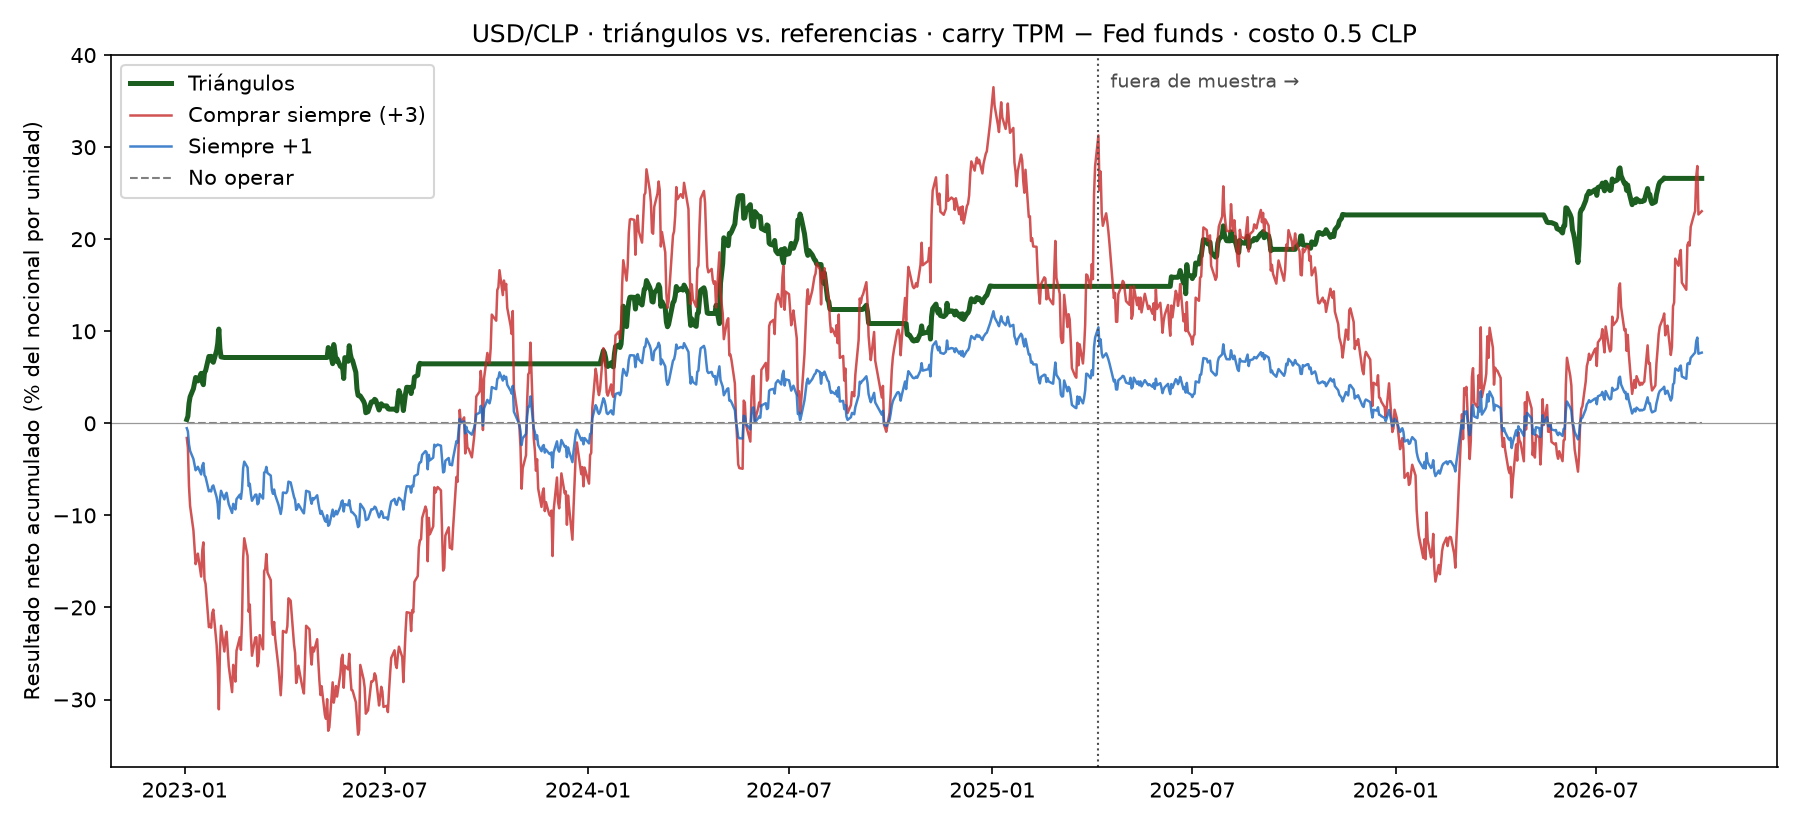
\includegraphics[width=\textwidth]{curva.png}}
  {\fbox{\parbox{0.9\textwidth}{\centering\vspace{2cm}Subir \texttt{curva.png}
  (generada por \texttt{estrategia.py})\vspace{2cm}}}}
\caption{Resultado neto acumulado contra las tres referencias. A la izquierda de
la línea punteada está la ventana de selección, donde se eligió la variante: ese
tramo no es evidencia fuera de muestra. A la derecha está el holdout.}\label{fig:curva}
\end{figure}

\paragraph{De dónde viene el resultado.} El neto se explica casi entero por
dirección: el bruto es $+13{,}8\%$, de los cuales $+10{,}5$ puntos vienen de
posiciones largas y $+3{,}3$ de cortas. Que gane por los dos lados importa: una
estrategia que solo gana comprada podría ser una apuesta disfrazada a que el dólar
sube. El carry casi no pesa ($-0{,}3\%$) por dos razones: la estrategia alterna
entre largo y corto, de modo que paga y recibe, y el diferencial de tasas bajó a
0,8 pp en el holdout. Las referencias pierden por lo contrario: el dólar casi no se
movió entre el inicio y el fin del tramo (de 989 a 973), así que no hubo ganancia
direccional que compensara el carry de estar largo todos los días.

\paragraph{Rotación.} Los costos suman $1{,}73\%$ con $c=0{,}5$ CLP: 32 unidades de
cambio de posición en 377 días, menos de una cada diez jornadas. Como vimos en la
§\ref{sec:compresion}, la ventaja por día es pequeña, así que la rotación baja es
condición para que exista resultado neto.

\paragraph{Riesgo.} La caída máxima es $-6{,}0\%$, frente a $-16{,}2\%$ de
siempre~+1. Hay dos razones. La estrategia está en cero el 59\% de los días, así que
no participa en muchas caídas. Y cuando está posicionada, el stop y la regla de
ruptura fallida cortan la pérdida antes de que se acumule. La curva tiene tramos
planos largos: son los períodos sin triángulo vigente.

\paragraph{Comparación con la ventana de selección.} En la ventana de selección la
variante obtuvo $+14{,}9\%$ con Sharpe 0,64; en el holdout, $+11{,}7\%$ con Sharpe
1,00. Que el Sharpe suba fuera de muestra es inusual y merece explicación, porque
lo normal es que caiga. Viene de 2025, un año de caída del dólar en que la
estrategia ganó por los dos lados ($+4{,}8$ puntos brutos largos y $+4{,}0$ cortos)
y estuvo fuera del mercado el 54\% de los días (Tabla~\ref{tab:subperiodos}). En
2026 el Sharpe vuelve a niveles parecidos a los de selección (0,66).

\subsection{Significancia}

\begin{table}[htbp]\centering\small
\begin{tabular}{@{}lccc@{}}
\toprule
Triángulos vs. & DM direccional ($p$) & DM cuadrático ($p$) & Bootstrap del neto ($p$) \\
\midrule
Comprar siempre (+3) & \textbf{0{,}045} & \textbf{0{,}000} & 0{,}316 \\
Siempre +1           & \textbf{0{,}045} & \textbf{0{,}000} & 0{,}118 \\
No operar            & \textbf{0{,}022} & 1{,}000 & 0{,}053 \\
\bottomrule
\end{tabular}
\caption{Contrastes unilaterales (H1: el triángulo es mejor). DM con varianza HAC
\citep{neweywest1987} y corrección de \citet{hln1997}; pérdida direccional: 0 si
acierta, 1 si falla, 0,5 si se abstiene; pérdida cuadrática con predicción puntual
igual a la posición por el retorno absoluto medio de la ventana de selección.
Bootstrap estacionario \citep{politisromano1994}, bloque medio de 10 días, 10.000
réplicas. Código: \ruta{experimentos/12_tests_finales.py}.}\label{tab:sig}
\end{table}

Las bases exigen dos pruebas porque responden preguntas distintas: si la
predicción es mejor y si el resultado económico es mayor. Una estrategia puede
predecir mejor y aun así no ganar más, por ejemplo si acierta en días de
movimientos chicos.

\textbf{Diebold-Mariano} \citep{dm1995} compara, día a día, la pérdida de nuestra
predicción con la de cada referencia y prueba si la diferencia promedio es
distinta de cero. Elegimos una pérdida direccional en que la abstención vale 0,5,
igual que una moneda al aire. Es una elección deliberadamente neutral: el modelo no
gana puntos por quedarse fuera, solo por acertar cuando entra. Si la abstención
valiera 0, la prueba premiaría no operar. Como las posiciones duran varios días,
las diferencias de pérdida están autocorrelacionadas; por eso la varianza es HAC.
La corrección de Harvey, Leybourne y Newbold ajusta la prueba para muestras
moderadas, donde el DM original tiende a rechazar de más.

La predicción supera a las tres referencias al 5\%. Con pérdida cuadrática supera
con holgura a comprar siempre y a siempre~+1, pero no a no operar. Es esperable: en
error cuadrático, predecir variación cero es muy difícil de batir, porque la
variación diaria promedio es cercana a cero y cualquier predicción distinta de
cero agrega error los días en que se equivoca.

\textbf{Bootstrap} pregunta si el resultado económico pudo salir por azar. Genera
10.000 historias alternativas remuestreando bloques de días consecutivos del
holdout y cuenta en cuántas la ventaja desaparece. Se remuestrean bloques, y no
días sueltos, para conservar la autocorrelación de las posiciones y la
agrupación de volatilidad. Contra no operar, $p=0{,}053$: si la estrategia no
tuviera valor, un resultado como este aparecería por azar cerca de 5 de cada 100
veces. Contra siempre~+1 y comprar siempre no alcanza significancia: esas
referencias son tan volátiles que, en 377 días, una diferencia de 13 puntos no
basta para descartar el azar.

Como la variante se eligió antes de abrir el holdout y el holdout se evaluó con un
solo modelo, estos $p$-valores no requieren ajuste por búsqueda múltiple.

\subsection{Robustez}\label{sec:robustez}

Un resultado robusto es uno que no depende de un supuesto particular. Probamos los
tres que más podrían moverlo: el costo, el período y el activo.

\begin{table}[htbp]\centering\small
\begin{tabular}{@{}lccccc@{}}
\toprule
Costo (CLP por dólar) & 0 & 0{,}25 & 0{,}5 & 1 & 2 \\
Aprox. en pb a 970 & 0 & 2,6 & 5,2 & 10,3 & 20,6 \\
\midrule
Neto holdout (\%) & 13{,}46 & 12{,}59 & \textbf{11{,}73} & 10{,}00 & 6{,}55 \\
\bottomrule
\end{tabular}
\caption{Sensibilidad a costos. Por extrapolación lineal, el neto llega a cero con
un costo cercano a 3,9 CLP por dólar (unos 40 pb).}\label{tab:costos}
\end{table}

\paragraph{Costo.} El neto cae de forma lineal con el costo, a razón de unos 3,5
puntos por cada peso adicional, porque la rotación no cambia. Con costos cuatro
veces el supuesto base sigue en $+6{,}6\%$.

\begin{table}[htbp]\centering\small
\begin{tabular}{@{}lccccc@{}}
\toprule
Tramo & Días & Dólar & Triángulos & Siempre +1 & Bootstrap vs. 0 ($p$) \\
\midrule
Abr--dic 2025 & 183 & $-8{,}3\%$ & \textbf{+7{,}8\%} & $-8{,}8\%$ & 0{,}051 \\
Ene--oct 2026 & 194 & +7{,}4\%   & +4{,}0\% & \textbf{+7{,}2\%} & 0{,}229 \\
\bottomrule
\end{tabular}
\caption{Resultado neto por sub-período del holdout.}\label{tab:subperiodos}
\end{table}

\paragraph{Sub-períodos.} La estrategia gana en los dos sub-períodos, con el dólar
bajando y subiendo. En 2025, con el dólar cayendo, gana $+7{,}8\%$ mientras
siempre~+1 pierde $-8{,}8\%$. En 2026, con el dólar subiendo, gana menos que
siempre~+1: es el costo de estar fuera del mercado buena parte de un año alcista.
Es un costo que aceptamos, porque la misma abstención es la que la protegió en 2025.

\begin{table}[htbp]\centering\small
\begin{tabular}{@{}lrrrl@{}}
\toprule
Ventana & Triángulos & Sharpe & Siempre +1 & Nota \\
\midrule
2005 -- 2018            & $-17{,}2\%$ & $-0{,}20$ & $-7{,}3\%$  & Bruto $+2{,}9\%$; pierde por costos y carry \\
18 oct 2019 -- 2022     & $+11{,}1\%$ & 0,30      & $+14{,}4\%$ & Período excluido \\
Ene 2023 -- abr 2025    & $+14{,}9\%$ & 0,64      & $+9{,}3\%$  & Ventana de selección \\
Abr 2025 -- oct 2026    & $+11{,}7\%$ & 1,00      & $-1{,}6\%$  & Holdout \\
\bottomrule
\end{tabular}
\caption{La variante final en todas las ventanas, con la misma contabilidad (carry
TPM $-$ Fed funds, costo 0,5 CLP).}\label{tab:todas}
\end{table}

\paragraph{Toda la historia.} La Tabla~\ref{tab:todas} muestra la variante final en
toda la historia disponible. En 2005--2018 pierde, y la §\ref{sec:compresion}
explica por qué: una ventaja de acierto modesta sobre movimientos pequeños, con un
costo que pesa más en términos porcentuales por el menor nivel del dólar.
Desde octubre de 2019 la estrategia es positiva en las tres ventanas, incluida la
excluida, que nunca se usó para elegir.

\paragraph{Otras monedas.} Si la lógica de órdenes acumuladas en niveles es
correcta, no debería ser exclusiva del peso chileno. Aplicamos la regla congelada,
sin cambiar ningún parámetro, a nueve cruces de la base entre enero de 2023 y
octubre de 2026 (Tabla~\ref{tab:monedas}). Para comparar en igualdad de
condiciones usamos la misma contabilidad en todos: sin carry, porque la base no
trae tasas locales de esos países, y con un costo de 5 pb por unidad de cambio de
posición, el equivalente al supuesto base del USD/CLP.

Es una prueba exigente por un motivo técnico. La base solo trae máximos y mínimos
para el USD/CLP; en las demás monedas las velas se reconstruyen con cierres. Eso
destruye la vela de rechazo, que necesita apertura y rango, y distorsiona los
pivotes, que necesitan máximos y mínimos reales. El efecto se puede medir en el
propio USD/CLP: con velas de cierre, el neto baja de $+28{,}4\%$ a $+4{,}8\%$ y el
tiempo con posición, de 44\% a 16\%. Lo que se prueba en las otras monedas es, por
lo tanto, una versión debilitada del detector.

\begin{table}[htbp]\centering\small
\begin{tabular}{@{}lrrrrr@{}}
\toprule
Moneda & Moneda en el período & Neto & Sharpe & \% días con posición & Siempre +1 \\
\midrule
USDCLP (OHLC real)    & $+13{,}3\%$ & $\mathbf{+28{,}4\%}$ & 0,80 & 43,8\% & $+15{,}6\%$ \\
USDCLP (solo cierres) & $+13{,}3\%$ & $+4{,}8\%$  & 0,27     & 15,7\% & $+15{,}6\%$ \\
\midrule
USDBRL & $-7{,}0\%$  & $+4{,}5\%$ & 0,16     & 21,9\% & $-4{,}6\%$ \\
USDMXN & $-7{,}6\%$  & $+1{,}2\%$ & 0,08     & 10,3\% & $-5{,}8\%$ \\
USDCOP & $-33{,}8\%$ & $+4{,}9\%$ & 0,33     & 6,1\%  & $-37{,}9\%$ \\
USDPEN & $-10{,}1\%$ & $-4{,}7\%$ & $-1{,}60$ & 3,5\% & $-10{,}0\%$ \\
USDZAR & $-2{,}7\%$  & $+6{,}0\%$ & 0,18     & 21,6\% & $+0{,}1\%$ \\
USDCNH & $-3{,}3\%$  & $+3{,}9\%$ & 1,01     & 8,4\%  & $-3{,}1\%$ \\
USDJPY & $+20{,}9\%$ & $+0{,}7\%$ & 0,07     & 7,3\%  & $+20{,}7\%$ \\
EURUSD & $+5{,}6\%$  & $+6{,}9\%$ & 0,46     & 9,3\%  & $+6{,}3\%$ \\
DXY    & $-2{,}6\%$  & $-4{,}3\%$ & $-0{,}55$ & 8,5\% & $-1{,}9\%$ \\
\bottomrule
\end{tabular}
\caption{La regla congelada aplicada a otras monedas, enero 2023 -- octubre 2026,
sin carry y con costo de 5 pb por unidad de cambio de posición. Fuera del USD/CLP
las velas se reconstruyen con cierres (la base no trae máximos y mínimos), lo que
debilita al detector: en el propio USD/CLP esa aproximación baja el neto de
$+28{,}4\%$ a $+4{,}8\%$. Neto positivo en 7 de 9 monedas; le gana a siempre +1 en
7 de 9. Código: \ruta{experimentos/10_triangulo_otras_monedas.py}.}\label{tab:monedas}
\end{table}

Aun con el detector debilitado, la regla tiene neto positivo en siete de las nueve
monedas y le gana a siempre~+1 en siete de las nueve. Ningún resultado individual
es significativo al 5\%, lo que es esperable con tan pocos días con posición: en la
mayoría de las monedas la regla opera menos del 10\% del tiempo. La lectura correcta
no es moneda por moneda, sino de conjunto. Si la regla no tuviera contenido, lo
esperable sería un resultado positivo en cerca de la mitad de las monedas; siete de
nueve es consistente con una ventaja pequeña y general, aunque las monedas se
mueven juntas y no son nueve pruebas independientes.

\paragraph{El caso del peso colombiano.} El COP es el caso más informativo. Es,
como el peso chileno, una moneda latinoamericana ligada a una materia prima, el
petróleo en vez del cobre. Y es la que tuvo la tendencia más fuerte del período:
el dólar cayó $33{,}8\%$ contra el peso colombiano. Una estrategia con sesgo
comprador habría sido destruida; siempre~+1 pierde $-37{,}9\%$. La regla, en
cambio, estuvo posicionada solo el 6\% de los días y terminó en $+4{,}9\%$, con una
caída máxima de $-6{,}3\%$ y el mejor Sharpe entre las monedas de la región
(0,33). Esto muestra dos cosas. Primero, que la estrategia no es una apuesta
disfrazada a que el dólar sube: en el mercado donde el dólar más cayó, no perdió.
Segundo, que la abstención es la que protege: el resultado no viene de acertar la
tendencia, sino de no pelear contra ella.

\paragraph{Dónde no funciona.} Pierde en dos casos. En el sol peruano opera solo
el 3,5\% de los días y su resultado descansa en muy pocas operaciones. El PEN es
una moneda de baja volatilidad con un banco central que interviene con frecuencia,
lo que es consistente con el argumento de la §\ref{sec:exclusion}: cuando la
autoridad forma el precio, los niveles dejan de importar. La lectura no es
concluyente, porque el yuan offshore, también una moneda administrada, da el mejor
Sharpe de la tabla (1,01). En el DXY pierde $-4{,}3\%$; es un índice de monedas
desarrolladas, no un cruce que se transe directamente. El caso del yen muestra el
costo de la abstención: el dólar subió $20{,}9\%$ y la regla capturó casi nada
($+0{,}7\%$), igual que en el USD/CLP de 2026 (Tabla~\ref{tab:subperiodos}).

\paragraph{Asimetría.} En los meses alcistas del holdout captura cerca de la mitad
del alza ($+9{,}8\%$ contra $+20{,}1\%$ de siempre~+1); en los bajistas se protege
quedando fuera ($+2{,}0\%$ contra $-17{,}3\%$; \ruta{experimentos/04d_meses_alcistas_bajistas.py}). Es el perfil que se busca en una
estrategia de abstención: renuncia a parte de las subidas a cambio de evitar casi
todas las caídas.

\paragraph{Horizonte del monitoreo.} En ventanas de 13 días hábiles del holdout,
el largo del monitoreo en vivo, gana en el 40\% de los casos, queda en cero en el
44\% y pierde en el 16\% (\ruta{experimentos/04e_ventanas_cortas.py}). Lo reportamos para fijar expectativas: en un período
tan corto, el resultado más probable después de ganar es no operar.

% ======================================================================
\section{Lectura de convicción}\label{sec:conviccion}

Las bases piden diagnosticar las jornadas de máxima exposición y las de
abstención. La pregunta de fondo es si la estrategia sabe cuándo sabe: si la
exposición alta coincide con mejores resultados y si los días en cero son días en
que no había nada que ganar.

\begin{table}[htbp]\centering\small
\begin{tabular}{@{}lrrrrr@{}}
\toprule
Exposición & Días & \% de días & Acierto & Neto & Siempre +1 esos días \\
\midrule
\multicolumn{6}{@{}l}{\textit{Holdout}}\\
$\pm3$ (máxima) & 6   & 1{,}6\%  & 66{,}7\% & +4{,}8\% & +1{,}7\% \\
$\pm1$ (media)  & 147 & 39{,}0\% & 58{,}5\% & +7{,}5\% & +1{,}7\% \\
0 (abstención)  & 224 & 59{,}4\% & --       & $-0{,}6\%$ & $-5{,}1\%$ \\
\addlinespace
\multicolumn{6}{@{}l}{\textit{Ene 2023 -- oct 2026 (incluye ventana de selección)}}\\
$\pm3$ (máxima) & 27  & 2{,}9\%  & 59{,}3\% & +15{,}1\% & $-1{,}1\%$ \\
$\pm1$ (media)  & 389 & 41{,}0\% & 54{,}0\% & +12{,}8\% & +8{,}2\% \\
0 (abstención)  & 533 & 56{,}2\% & --       & $-1{,}3\%$ & +0{,}6\% \\
\bottomrule
\end{tabular}
\caption{Resultado por nivel de exposición. El neto en abstención corresponde al
costo de cerrar posiciones, que se registra el día en que la posición pasa a cero.}
\label{tab:conviccion}
\end{table}

\paragraph{Máxima exposición.} La estrategia entra en $\pm3$ muy pocas veces: 6
días en el holdout y 27 en todo el período. Es una decisión de diseño: el retest
exige que ocurran tres cosas en orden (ruptura, regreso al borde y reanudación), y
cuando ocurren la evidencia es más fuerte que en una ruptura sola. Esos días
aciertan más que el promedio (67\% en el holdout, 59\% en todo el período) y ganan
en promedio 81 pb por día en el holdout, frente a 5 pb de los días en $\pm1$. La
diferencia no es solo de tamaño: dividido por tres, cada unidad en $\pm3$ gana 27
pb por día, más de cinco veces lo que gana en $\pm1$. Con tan pocos días no es una
prueba estadística, pero el patrón se repite en los dos tramos: a mayor exposición,
mayor acierto y mayor ganancia por unidad.

\paragraph{Exposición media.} Es el grueso de la actividad. Acierta 58,5\% en el
holdout y aporta $+7{,}5\%$. Su ganancia por día es pequeña, como anticipa la
§\ref{sec:compresion}, pero se repite en muchos días.

\paragraph{Abstención.} Estar en cero es una decisión del modelo, no una falla. En
el holdout, siempre~+1 perdió $-5{,}1\%$ en los días en que la estrategia estuvo
fuera: esa pérdida se evitó. En todo el período, siempre~+1 ganó $+0{,}6\%$ en esos
días: lo que se dejó pasar es casi nada. El movimiento absoluto promedio del dólar
en los días de abstención del holdout (63 pb) no es menor que en los días en
$\pm1$ (48 pb): el modelo no se abstiene porque el mercado esté quieto, sino
porque no hay estructura que le dé una dirección.

\begin{table}[htbp]\centering\small
\begin{tabular}{@{}lrrrr@{}}
\toprule
Caso & Días & Acierto & Neto & Neto prom. (pb/día) \\
\midrule
\texttt{RETEST\_ABAJO}   & 6   & 66{,}7\% & +9{,}6\%  & 160 \\
\texttt{RETEST\_ARRIBA}  & 21  & 57{,}1\% & +5{,}5\%  & 26 \\
\texttt{RUPTURA\_ARRIBA} & 260 & 55{,}0\% & +7{,}4\%  & 3 \\
\texttt{RUPTURA\_ABAJO}  & 116 & 52{,}6\% & +4{,}4\%  & 4 \\
\texttt{BASE}            & 10  & 50{,}0\% & +2{,}7\%  & 27 \\
\texttt{TECHO}           & 3   & 33{,}3\% & $-1{,}7\%$ & $-56$ \\
\bottomrule
\end{tabular}
\caption{Resultado por caso, enero 2023 -- octubre 2026 (incluye la ventana de
selección).}\label{tab:casos}
\end{table}

Las rupturas son las más frecuentes (376 de 416 días con posición) y aportan 11,8
puntos del resultado; los retests aportan 15,1 puntos en apenas 27 días. Los
rebotes en el techo son pocos y pierden; con tres días no hay base para
eliminarlos sin caer en sobreajuste, y no los eliminamos. Eliminar una regla porque
perdió en tres días sería exactamente el tipo de decisión que el protocolo prohíbe.

% ======================================================================
\section{Estrategia automatizada}\label{sec:auto}

El repositorio
(\href{https://github.com/jdiazce/quantclp-torneo}{\texttt{github.com/jdiazce/quantclp-torneo}})
contiene la estrategia lista para ejecutarse, con la estructura habitual de una
estrategia algorítmica \citep{hilpisch2020}. Un solo script, \texttt{estrategia.py},
lee la base, recalcula la señal de cada día con la serie truncada en esa fecha y
produce tres salidas en \texttt{salidas/}:
\begin{itemize}
  \item \texttt{senal\_del\_dia.json}: dirección esperada, posición, caso, tipo de
        triángulo, probabilidad estimada de alza y convicción.
  \item \texttt{curva.png}: resultado neto acumulado contra las tres referencias
        (Figura~\ref{fig:curva}).
  \item \texttt{historial.csv}: posición, caso y resultado de cada día.
\end{itemize}
Además imprime la lectura de convicción de la §\ref{sec:conviccion}. Recalcular
cada día con la serie truncada es más lento que calcular todo de una vez, pero
garantiza que la historia que mostramos es exactamente la que la estrategia habría
producido en tiempo real.

\paragraph{Probabilidad estimada.} La probabilidad de alza es la frecuencia de
acierto de cada nivel de exposición en la ventana de selección, calculada solo con
datos previos al holdout (Tabla~\ref{tab:prob}). Si la posición es positiva,
$P(\text{sube})$ es el acierto del nivel; si es negativa, uno menos el acierto; si
es cero, la frecuencia de alzas de la ventana. Es una probabilidad empírica, no la
salida de un modelo estadístico, y es deliberadamente modesta. Que la señal más
frecuente tenga una probabilidad de apenas 51\% es coherente con lo que dicen las
bases: la ventaja no está en predecir mucho mejor que el azar, sino en saber cuándo
apostar.

\begin{table}[htbp]\centering\small
\begin{tabular}{@{}lrrrr@{}}
\toprule
Nivel & Días en selección & Acierto & $P(\text{sube})$ si $+$ & $P(\text{sube})$ si $-$ \\
\midrule
$\pm1$ & 242 & 51{,}2\% & 51{,}2\% & 48{,}8\% \\
$\pm3$ & 21  & 57{,}1\% & 57{,}1\% & 42{,}9\% \\
0      & --  & --       & \multicolumn{2}{c}{50{,}9\% (frecuencia de alzas)} \\
\bottomrule
\end{tabular}
\caption{Probabilidad estimada de alza según el nivel de la señal, enero 2023 --
abril 2025.}\label{tab:prob}
\end{table}

\paragraph{Ejemplo.} Con el cierre del 6 de octubre de 2026 (973,95), la señal es
\emph{sin dirección}, posición 0 y $P(\text{sube})=50{,}9\%$. Hay tres triángulos
detectados (uno descendente y dos simétricos, formados entre febrero y marzo), pero
todos pasaron su ápice y están vencidos.

\paragraph{Ejecución.} Con la base en \texttt{data/}, \texttt{python estrategia.py};
con una base actualizada en otra ruta, \texttt{python estrategia.py
ruta/base.xlsx}. Durante el monitoreo en vivo (13 de noviembre -- 1 de diciembre)
se ejecuta cada día al cierre sin modificar el código ni los parámetros.

\begin{table}[htbp]\centering\small
\begin{tabular}{@{}ll@{}}
\toprule
Ruta & Contenido \\
\midrule
\texttt{estrategia.py}  & Estrategia automatizada: señal del día, curva y convicción \\
\texttt{src/}           & Detector y reglas (\texttt{triangulos.py}); probit ordenado de los experimentos \\
\texttt{experimentos/}  & Scripts de cada prueba, \texttt{registro\_experimentos.csv} y tests finales \\
\texttt{informe/}       & Este documento \\
\texttt{data/}          & Aquí va la base del torneo (no se incluye: datos Bloomberg) \\
\texttt{salidas/}       & Se genera al ejecutar \texttt{estrategia.py} \\
\bottomrule
\end{tabular}
\caption{Estructura del repositorio.}
\end{table}

% ======================================================================
\section{Limitaciones}\label{sec:limitaciones}

\begin{itemize}
  \item \textbf{Depende del régimen.} La variante final pierde $-17{,}2\%$ en
        2005--2018 y, en ese período, ninguna de las 24 variantes tiene neto
        positivo: el \emph{reality check} de \citet{white2000} no rechaza
        ($p=0{,}91$). La §\ref{sec:compresion} da una explicación, pero no
        afirmamos que la ventaja sea una propiedad permanente del peso.
  \item \textbf{Valor económico contra siempre~+1.} No es significativo
        ($p=0{,}12$). La predicción sí lo es.
  \item \textbf{Búsqueda.} La variante se eligió entre 24, antes de abrir el
        holdout. El resultado en la ventana de selección está optimizado; el del
        holdout no.
  \item \textbf{Muestra con posición.} 153 días con exposición en el holdout, 6
        de ellos en $\pm3$.
  \item \textbf{Efecto compresión.} La evidencia sobre dirección es modesta
        ($p=0{,}055$ en 2005--2018) y no se observa en el holdout, con solo 8
        casos.
  \item \textbf{Períodos en cero.} En horizontes cortos el modelo puede pasar
        semanas sin operar. En el monitoreo en vivo es posible que el resultado
        sea cero.
  \item \textbf{Shocks de política.} Una intervención cambiaria como la de 2022
        mueve el precio por razones que el detector no ve. El stop limita la
        pérdida, pero no la elimina.
  \item \textbf{Precio de ejecución.} Suponemos que se opera al cierre de
        Santiago con un costo fijo. Un costo mayor reduce el resultado, pero se
        necesitan cerca de 3,9 CLP por dólar para eliminarlo.
\end{itemize}

% ======================================================================
\section{Conclusión}

Una regla simple, que un trader puede explicar en una frase, obtiene $+11{,}7\%$
neto en 18 meses que no vio durante su desarrollo, con un tercio de la caída
máxima de siempre~+1 y fuera del mercado la mayor parte del tiempo. Su predicción
direccional supera a las tres referencias, y su resultado sobrevive a costos
cuatro veces mayores que el supuesto base.

¿Bastan la compresión y los triángulos para predecir el dólar? La compresión sola,
no: en el peso no anuncia movimientos más grandes y su efecto sobre la dirección es
modesto. Lo que la vuelve útil es combinarla con niveles concretos, confirmación y
disciplina para quedarse fuera. La estrategia no gana por acertar más, sino por
saber cuándo no apostar y cuándo apostar fuerte: cuando se abstiene evita pérdidas,
y cuando entra con máxima convicción acierta más y gana más por unidad.

Es también una estrategia honesta sobre sus límites. Funciona en el régimen
reciente del peso y no en 2005--2018, su valor económico contra siempre~+1 no es
estadísticamente significativo y puede pasar semanas sin operar. Reportamos todo lo
que probamos, lo que falló y los períodos en que la regla no funciona, porque una
estrategia que se puede defender vale más que una que solo se ve bien.

% ======================================================================
\appendix
\section{Registro de experimentos}\label{app:registro}

\begin{table}[htbp]\centering\small
\begin{tabular}{@{}llrrl@{}}
\toprule
Experimento & Período & Entradas & Neto (\%) & Nota \\
\midrule
02 Triángulos piloto     & 2023 -- mar 2025 & 2  & $-3{,}1$ / $+0{,}1$ & Primera versión \\
03 Grilla de triángulos  & 2005 -- 2018     & 24 & $-48{,}7$ a $-12{,}8$ & RC: $p=0{,}91$ vs. 0 \\
04 Selección             & 2023 -- mar 2025 & 2  & $+14{,}8$ / $-6{,}5$ & Mejor / peor invertida \\
05 Probit ordenado       & 2023 -- mar 2025 & 7  & $-8{,}5$ a $-2{,}3$ & Fijo y walk-forward \\
06 Doble validación      & 2023 -- mar 2025 & 6  & $-1{,}0$ a $+15{,}3$ & Descartado por simplicidad \\
07--08 Brecha post-cierre & 2023 -- mar 2025 & 4 & $-11{,}0$ a $+3{,}3$ & Se rompe en 2023+ \\
09 Tendencia             & 2023 -- mar 2025 & 4  & $-25{,}2$ a $+13{,}8$ & Registrado después \\
\midrule
04b--c Holdout           & abr 2025 -- oct 2026 & 4 & $+11{,}7$ & Un modelo, dos aperturas \\
\midrule
04d Meses por signo      & abr 2025 -- oct 2026 & \completar{} & -- & Modelo congelado \\
04e Ventanas de 13 días  & abr 2025 -- oct 2026 & \completar{} & -- & Modelo congelado \\
10 Otras monedas         & 2023 -- oct 2026 & \completar{} & -- & Regla sin cambios \\
12 Tests finales         & abr 2025 -- oct 2026 & \completar{} & -- & DM y bootstrap \\
13 Compresión            & 2005 -- 2026     & 3  & -- & Descriptivo \\
\midrule
Total                    &                  & \completar{} & & \\
\bottomrule
\end{tabular}
\caption{Resumen del registro. Cada fila del archivo
\texttt{registro\_experimentos.csv} tiene fecha, período, parámetros y resultado.
Los experimentos 02 a 06 usan carry NDF (nota al pie de la §\ref{sec:reglas}). Los
experimentos 04d, 04e, 10, 12 y 13 se corrieron después de evaluar el holdout y
no modifican el modelo.}
\end{table}

% ======================================================================
\begin{thebibliography}{99}\small
\bibitem[Bollerslev(1986)]{bollerslev1986}
Bollerslev, T. (1986). Generalized autoregressive conditional heteroskedasticity.
\textit{Journal of Econometrics}, 31(3), 307--327.

\bibitem[Diebold y Mariano(1995)]{dm1995}
Diebold, F.~X. y Mariano, R.~S. (1995). Comparing predictive accuracy.
\textit{Journal of Business \& Economic Statistics}, 13(3), 253--263.

\bibitem[Edwards et~al.(2018)]{edwards2018}
Edwards, R.~D., Magee, J. y Bassetti, W.~H.~C. (2018). \textit{Technical Analysis
of Stock Trends} (11.\textsuperscript{a} ed.). CRC Press.

\bibitem[Harvey et~al.(1997)]{hln1997}
Harvey, D., Leybourne, S. y Newbold, P. (1997). Testing the equality of prediction
mean squared errors. \textit{International Journal of Forecasting}, 13(2), 281--291.

\bibitem[Hilpisch(2020)]{hilpisch2020}
Hilpisch, Y. (2020). \textit{Python for Algorithmic Trading}. O'Reilly.

\bibitem[Lo(2004)]{lo2004}
Lo, A.~W. (2004). The adaptive markets hypothesis. \textit{Journal of Portfolio
Management}, 30(5), 15--29.

\bibitem[Lo et~al.(2000)]{lmw2000}
Lo, A.~W., Mamaysky, H. y Wang, J. (2000). Foundations of technical analysis.
\textit{Journal of Finance}, 55(4), 1705--1765.

\bibitem[López de Prado(2018)]{lopezdeprado2018}
López de Prado, M. (2018). \textit{Advances in Financial Machine Learning}. Wiley.

\bibitem[Menkhoff y Taylor(2007)]{menkhoff2007}
Menkhoff, L. y Taylor, M.~P. (2007). The obstinate passion of foreign exchange
professionals: technical analysis. \textit{Journal of Economic Literature}, 45(4),
936--972.

\bibitem[Newey y West(1987)]{neweywest1987}
Newey, W.~K. y West, K.~D. (1987). A simple, positive semi-definite,
heteroskedasticity and autocorrelation consistent covariance matrix.
\textit{Econometrica}, 55(3), 703--708.

\bibitem[Osler(2000)]{osler2000}
Osler, C.~L. (2000). Support for resistance: technical analysis and intraday
exchange rates. \textit{Federal Reserve Bank of New York Economic Policy Review},
6(2), 53--68.

\bibitem[Osler(2003)]{osler2003}
Osler, C.~L. (2003). Currency orders and exchange rate dynamics: an explanation
for the predictive success of technical analysis. \textit{Journal of Finance},
58(5), 1791--1819.

\bibitem[Politis y Romano(1994)]{politisromano1994}
Politis, D.~N. y Romano, J.~P. (1994). The stationary bootstrap. \textit{Journal
of the American Statistical Association}, 89(428), 1303--1313.

\bibitem[White(2000)]{white2000}
White, H. (2000). A reality check for data snooping. \textit{Econometrica}, 68(5),
1097--1126.
\end{thebibliography}

\end{document}